\documentclass{beamer}
\usepackage{graphicx}
\usepackage{hyperref}
\usepackage{pdfpages}
\usepackage{array}
\begin{document}
\begin{frame}
\begin{center}
{\Large
Lessons Learned and New Perspectives \\
From Dean and Provost to aspiring Data Scientist
}
\end{center}

\vskip 1in
{\small
Jeremy Teitelbaum \\
October 18, 2018 \\
University of Wisconsin -- Madison
}
\end{frame}
\begin{frame}{Outline}
\begin{enumerate}
\item Lessons from administration
\begin{enumerate}
\item The good and bad of life as an administrator
\item Some thoughts about math departments from the perspective of higher administration
\end{enumerate}
\item New challenges at the Jackson Laboratories (JAX)
\begin{enumerate}
\item A brief introduction to JAX and the people who work there
\item Two problems of interest to the genomicists at JAX
\end{enumerate}
\item Some comments on graduate education (in general, and in mathematics)
\end{enumerate}
\end{frame}

\begin{frame}{Some personal thoughts on administration: Likes}
\begin{itemize}
\item Opportunity to be a force for good
  \item Work with a diverse group of people (intellectual diversity within the unversity; skilled non-academics; more normal gender diversity)
  \item Challenging (in fact, often intractable) problems
  \item Teamwork
    \item Use different skills than in research (interpersonal skills and empathy; communication)
\end{itemize}
\end{frame}

\begin{frame}{Dislikes}
\begin{itemize}
\item Less control over your time
  \item Constant need to manage up and down
  \item Stress
  \item Frustration
\end{itemize}
\end{frame}

\begin{frame}{Thoughts on academia}
  \begin{itemize}
  \item Academic careers are long.  Some people get stuck and get unhappy, then make everyone around them unhappy. Math particularly impermeable.
  \item Academic institutions are far too tolerant of bad behavior; people work around it and manage it.
  \item Lack of diversity and failure to make progress on it taints the enterprise.  Deep problems and no progress on them.
  \end{itemize}
\end{frame}

\begin{frame}{Jackson Labs}
  \begin{itemize}
  \item Founded in 1929 in Bar Harbor, Maine.
  \item World center for mouse genetics.  Supplier of laboratory  mice to the world -- 3M per year shipped world wide.
  \item Mouse genome database contains enormous amount of information on mice and their genetic profiles.
  \item 26 Nobel Prizes associated with JAX.
  \item New CT facility has 350 employees focused on precision medicine and cancer.
  \item About 90 million in NIH funding and 256M per year in mouse business.
  \end{itemize}
\end{frame}
\begin{frame}{JAX, cont'd}
  \begin{itemize}
  \item 30 faculty: 10:1 staff to faculty ratio.  Huge IT infrastrcture, imaging and sequencing base staffed by Ph.D.'s.
  \item LOTS of jobs.  Very diverse group of postdocs and research scientists including biologists, physicsts, computer scientists and some mathematicians.
  \item Very different than a university because they are GROWING and HIRING all the time.
  \item JAX, or places like it, worth thinking about for math Ph.D.'s if they want to do science as an alternative to NSA or Finance jobs outside academia.
  \end{itemize}
\end{frame}
        
  
\begin{frame}{1. Diagnosis and the Human Phenotype Ontology}
\begin{block}{}
A human mendelian disease is a disorder that is attributable to a mutation in a single gene.  Such diseases
are inherited according to the classical laws of mendelian genetics.  \textit{Sickle cell anemia}, caused by the change of 
a single nucleotide on chromosome 11, is an example of such a disease.
\end{block}
\begin{block}{}
The website \href{http://www.omim.org}{Online Mendelian Inheritance in Man} summarizes information
about ``Mendelian Diseases''  It identifies over 5000 conditions for which the cause is a change in a single gene.
Of the over 30000 genes in humans, 3500 genes have known mutations that cause disease.
\end{block}
\begin{block}{}
Many of these diseases cause a constellation of abnormalities making them difficult to diagnose.
\end{block}
\end{frame}
\begin{frame}
\begin{block}{}
  The Human Phenotype Ontology (HPO) is a directed acyclic graph $HPO$
  nodes are 'symptoms.'  More specific symptoms are child nodes of
  more general ones.  The ontology is carefully curated to reflect
  standard medical terminology.
\end{block}
\begin{block}{}
The HPO was initially constructed by Peter Robinson and his group at
Charite hospital in Berlin.  Robinson is now at JAX.
\end{block}
\end{frame}
\begin{frame}
A disease $d$ is characterized by a finite set of symptoms (nodes of the HPO) and therefore by its spanning
subtree $HPO(d)\subset HPO$.
\begin{center}
Angleman's Disease
\end{center}
\begin{tabular}{m{1.5in}m{3in}}
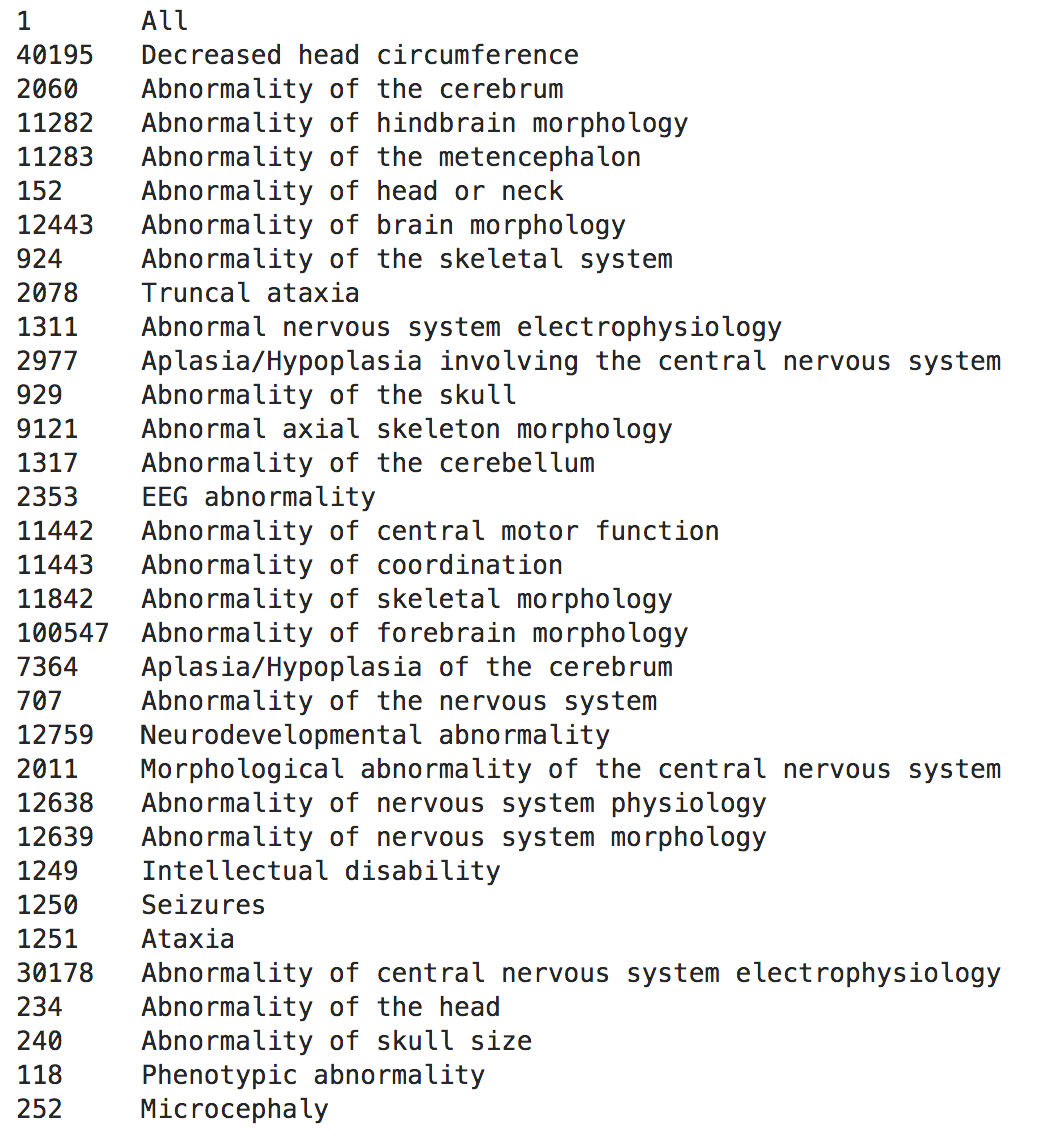
\includegraphics[width=1.5in]{angleman_symptoms.png} & 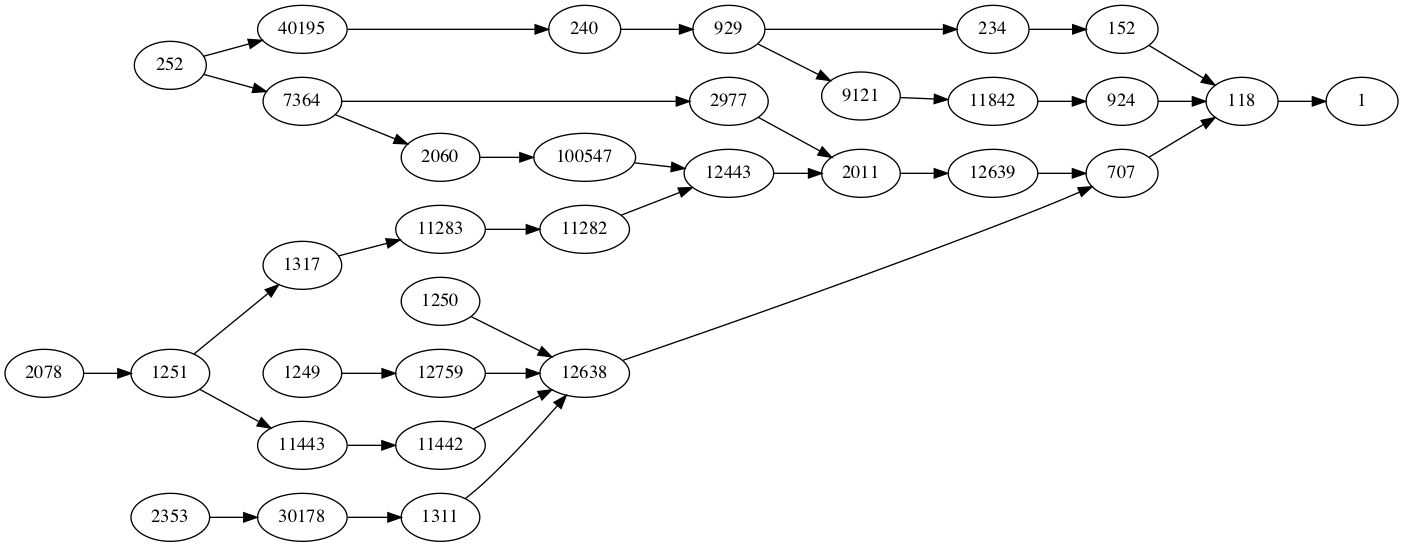
\includegraphics[width=2.5in]{anglemanI.png}\cr
\end{tabular}
\end{frame}
\begin{frame}
A doctor examining a patient identifies a list of symptoms $S$, which in turn determine a spanning subtree
$HPO(S)$.

\begin{problem} Given a symptom subtree $HPO(S)$, find a set of diseases (subtrees $HPO(D)$), scored by some type of likelihood measure, that are consistent with the symptoms.
\end{problem}

Complications:
\begin{itemize}
\item Doctor may give more general version of a symptom, rather than the most specific one.
\item Doctor may miss some symptoms, or they may be rare even among people with a disease.
\item Doctor may add unrelated symptoms.
\end{itemize}
\end{frame}
\begin{frame}{Semantic Similarity}
  In 1995 Resnick proposed a similarity measure for ontologies based on the ``information content'' of a node.
  \begin{itemize}
  \item Given a node (symptom) $m$, let $\mathcal{A}(m)$ be the set of diseases that are associated with that node -- meaning some descendant of that node is a specific symptom of the disease.
  \item Assign weights to the edges of the DAG by setting the weight of $n\to m$ to be $\log |\mathcal{A}(m)|-\log |\mathcal{A}(n)|$.
  \item The information content $IC(n)$  of a node $n$ is the sum of the weights of the edges from the node to the root (along any path).
  \end{itemize}

  \end{frame}
\begin{frame}
\begin{block}{}
  The Resnick similarity between two sub-DAG's $X$ and $Y$ is $(H(X,Y)+H(Y,X))/2$
  where
  $$
  H(X,Y)=\frac{1}{|X|}\sum_{x\in X} \max_{y\in Y} IC(z(x,y))
  $$
  where $z$ is the common ancestor of $x$ and $y$ with the greatest $IC$.
\end{block}
\begin{block}{}
  \textit{A new method to measure the semantic similarity from query phenotypic abnormalities to diseases based on the human phenotype ontology}, in \textit{BMC Bioinformatics 2018}, lists six other
  'distance measures' between subtrees of a DAG, and adds a new one.
  There are many others.
\end{block}
\end{frame}
\begin{frame}
More sophisticated models under development:
\begin{enumerate}
\item incorporate information about the relative frequencies of symptoms in patients with the disease
\item attempt to incorporate information about genetic variants into the diagnosis.
\end{enumerate}

Common validation technique is to test against simulated data.
\begin{problem}
Formally characterize the differences, strengths, weaknesses of these different approaches.
\end{problem}
\end{frame}
\begin{frame}{2. Analysis of single cell RNA experiment data}
  Two seconds on human molecular genetics.
\begin{center}
  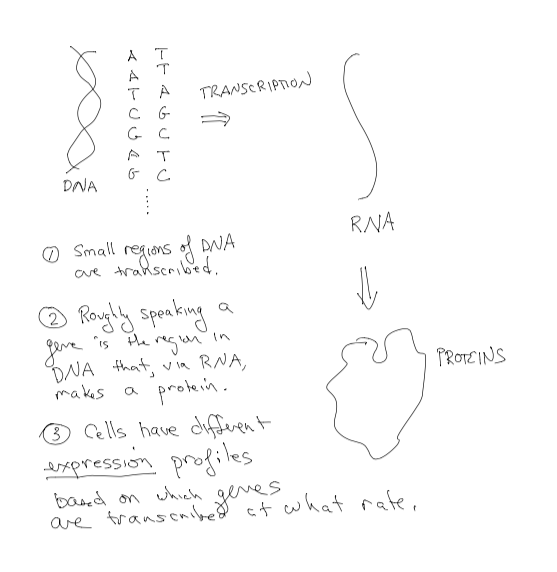
\includegraphics[width=3in]{dna.png}
\end{center}
\end{frame}
\begin{frame}{RNA-seq}
\begin{itemize}
\item  In 'Bulk RNA sequencing' (RNA-seq) researchers take a sample of a particular tissue type, sequence the RNA in the sample by cutting it up into pieces and aligning the pieces against a reference genome.
\item They count the fragments of RNA that line up against a particular gene and use that as a measure of the relative activation level of that particular gene AVERAGED OVER THE CELLS IN THE SAMPLE.
\item Typical experiments:
  \begin{itemize}
  \item Take cells before and after treatment with a drug and look to see if the expression profile has changed.
  \item Compare expression profile of normal and cancer cells and look for genes that are amplified or repressed in cancer; these might suggest biochemical pathways for drug targeting.
  \end{itemize}
\end{itemize}
\end{frame}
\begin{frame}
  \begin{itemize}
        \item
  Typical experiment might have 3 or 4 controls, 3 or 4 treatment cases, and 30000 genes.  So for Bulk RNA sequencing the problem is to identify which of those 30000 genes differ between the controls and treatment cases.  
\item Although this technology is perhaps only 10 years old, it is now standard and there are established techniques for this.
\end{itemize}
\end{frame}
\begin{frame}{Single Cell RNA-Seq}
  In single cell RNA-seq, \textit{individual cells} are captured to obtain a cell by cell expression profile.
  \begin{itemize}
  \item Cells are caught in droplets and RNA in each droplet gets a unique sequence identifying the droplet attached; plus each RNA molecule gets a unique sequence identifying the molecule.
  \item Then these pieces are amplified (replicated many times).  The resulting 'library' gets sequenced.
  \item In this way one can count the number of RNA molecules from each gene in each cell.
  \item Some nice, elementary use of error correcting codes takes place here.'
  \end{itemize}
\begin{center}
  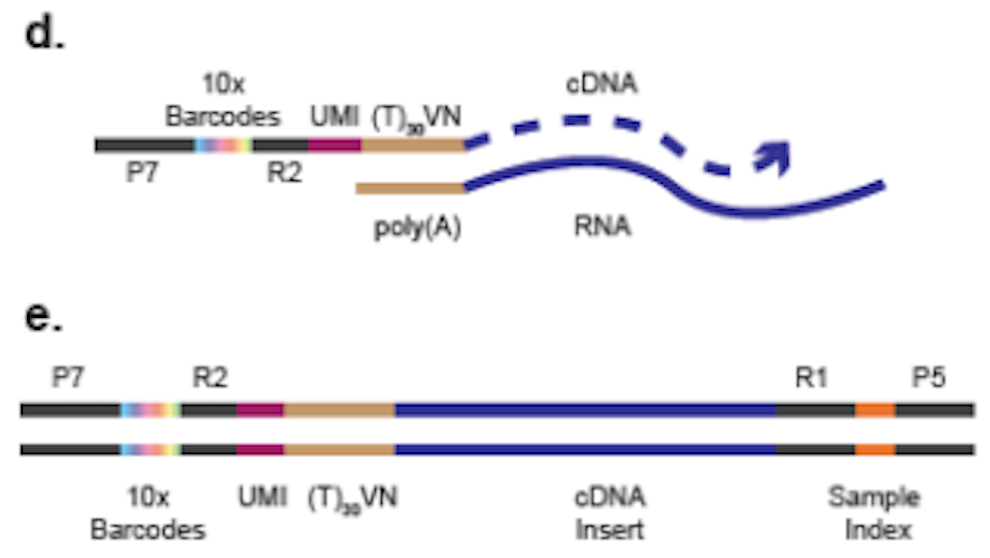
\includegraphics[width=1.75in]{10XSingleCellDetail.png}
\end{center}
\end{frame}
\begin{frame}
\begin{center}
  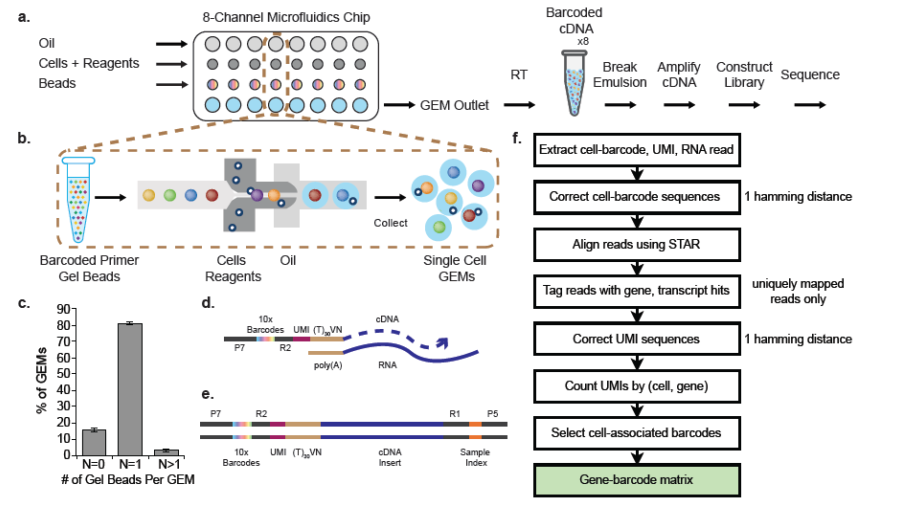
\includegraphics[width=3in]{10xSingleCellOverview.png}

  10x Genomics droplet high-throughput single cell platform
\end{center}
\end{frame}
\begin{frame}{Single Cell Data}
\begin{block}{}
  The output from a single cell experiment is an $N\times K$ sparse integer matrix.  Here $N$, the number of cells, could range from a few hundred to a few million, and $K$, the number of genes, is on the order of $30000$.  The $(i,j)$-th entry of the matrix is the activation level of gene $j$ in cell $i$.
\end{block}
\begin{block}{}
  Goals for these experiments are:
  \begin{itemize}
  \item Obtain fine structure among classes of cells based on their expression profiles.
  \item Understand developmental history and reconstruct development.
  \item Understand tumor heterogeneity and its relationship to chemotherapy response (*)
  \item Many other things....
  \end{itemize}
\end{block}
\end{frame}
\begin{frame}{Outline of Analysis}
  \begin{enumerate}
  \item Clean up the data by throwing out cells with few detected genes and genes that hardly ever show up.
  \item Normalize the data by cell to account for the different levels of sequencing success.
  \item Do a first round of dimensionality reduction by identifying genes that show a lot of variance
  \item Use a second round of dimensionality reduction to two or three dimensions (PCA, tSNE, or UMAP)
  \item Cluster the results
  \item Look at the gene profiles of each cluster to try to find genetic markers for each cluster.
  \item Figure out the biological implications.
  \end{enumerate}
  
  

  
\end{frame}
\begin{frame}
  \begin{center}
      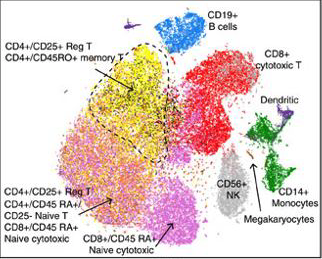
\includegraphics[width=3in]{blood.png}

      Immune cell types in blood from \textit{Massively parallel digital transcriptional profiling of single cells} by Zheng, et. al., Nature Comm. 8, 2017.
\end{center} 
\end{frame}

\begin{frame}{Challenges with scRNA data}
  \begin{block}{Sparsity}
    There is considerable activity in the literature over some basic questions about how to analyze single cell data.
    Much of this comes from the sparsity of the data.
    \begin{enumerate}
          \item How to distinguish between genes that have low (or zero) expression and
            genes that show up with zero expression for technical reasons?
          \item How to properly normalize the data by cell when there is so much variation in the total count per cell?
          \item How to identify subpopulations within the data when the subpopulations could be distinguished by differential expression of only a very small number of the 30000 genes being profiled?
          \end{enumerate}
\end{block}
\end{frame}

\begin{frame}
  More questions:
        \begin{enumerate}
        \item What is the proper statistical model for this data?  I count more than 10 proposals that have been published in different studies.
        \item How sensitive are the common dimensionality reduction algorithms used for clustering to the different choices one makes for normalization and to the possible dropout of some values?
        \item How to integrate this data with 'bulk' sequencing data or other types of data.
        \end{enumerate}
\end{frame}
\begin{frame}{Very recent: random matrix theory applied to single cell data}
\begin{block}{}
The paper \textit{Quasi-universality in single-cell sequencing data}, by Aparicio, Bordyuh, Blumberg, and Rabadan, looks
at the spectra of matrices arising from single cell experiments through the lens of random matrix theory.
\end{block}
\begin{block}{}
One formulates a 'null hypothesis' that the matrix of data is random, and and can identify a signal by identifying the the extent that the eigenvalue distribution of the correlation matrix differs from the universal distribution that one expect.
\end{block}
\begin{block}{}
The sparsity of the data matrices is an obstacle to this and needs to be accounted for.
\end{block}
\end{frame}
\begin{frame}{More on random matrices and single cell data}
From the paper cited above.
\begin{center}
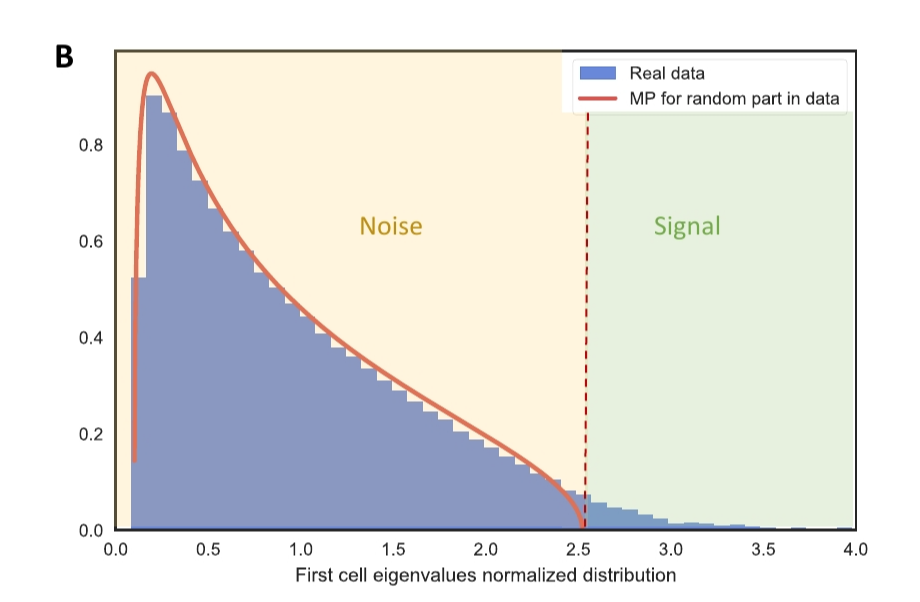
\includegraphics[width=4in]{RMT2.png}
\end{center}
\end{frame}
\begin{frame}{Structure of single cell data from random matrix perspective}
From the paper cited above.
\begin{center}
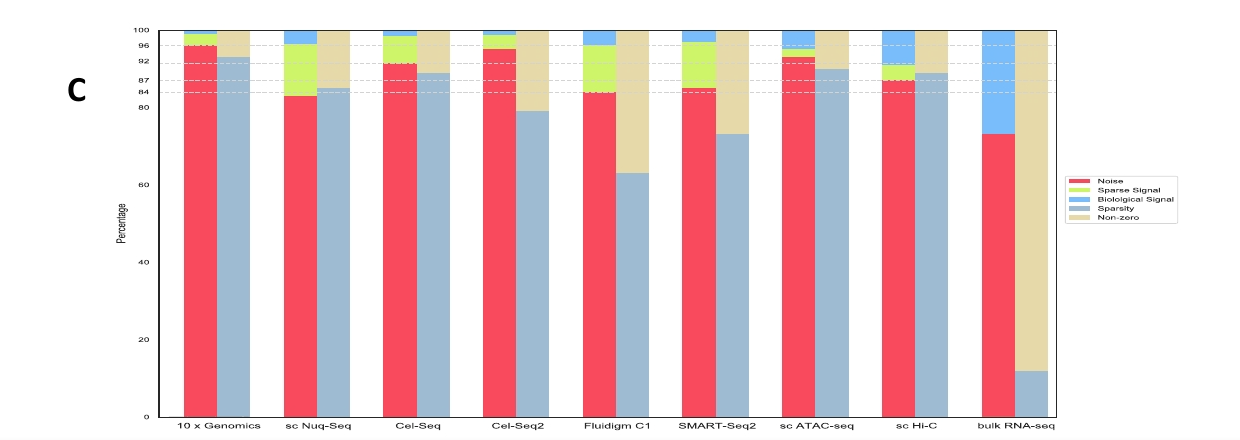
\includegraphics[width=4.5in]{RMT1.png} 
\end{center}
\end{frame}


\begin{frame}{Some thoughts about graduate education in math}

  Goal is to train successful research mathematicians, but students need to protect their economic mobility as a hedge against exploitation.  Not clear what long-term future of academic jobs will be.

  \begin{itemize}
  \item (Not a radical idea) Insist on knowledge of programming.
    \item Include some statistics in the core curriculum for mathematicians.
      \item Find a way to include group projects in the curriculum.
      \item Math in general is pretty good about time-to-degree but in academia in general students have to get through fast.
      \end{itemize}
      \end{frame}
  
\end{document}



%%% Local Variables:
%%% mode: latex
%%% TeX-master: t
%%% End:
